\documentclass[conference]{IEEEtran}
\usepackage{cite}
\usepackage{amsmath,amssymb,amsfonts}
\usepackage{algorithmic}
\usepackage{graphicx}
\usepackage{textcomp}
\usepackage{xcolor}
\usepackage[shortcuts,acronym]{glossaries}

\def\BibTeX{{\rm B\kern-.05em{\sc i\kern-.025em b}\kern-.08em
    T\kern-.1667em\lower.7ex\hbox{E}\kern-.125emX}}
    
\makeglossaries
\newacronym[plural= API's, firstplural=Application Programming Interfaces]{api}{API}{Application Programming Interface}
\newacronym{rest}{REST}{Representational State Transfer}
\newacronym{gdpr}{GDPR}{General Data Protection Regulation}
\newacronym{oas}{OAS}{OpenAPI Specification}

\begin{document}
\title{Working Title - Transparency and Records of processing in agile DevOps:
Towards a GDPR-focused tracing Toolbox
% {\footnotesize \textsuperscript{*}Note: Sub-titles are not captured in Xplore and should not be used}
}

\author{
    \IEEEauthorblockN{Daniel Habenicht}
    \IEEEauthorblockA{\textit{Masters Student} \\
    \textit{TU Berlin}\\
    Berlin, Berlin \\
    email address or ORCID}
\and
    \IEEEauthorblockN{Lucas Kettenmann}
    \IEEEauthorblockA{\textit{Masters Student} \\
    \textit{TU Berlin}\\
    Berlin, Berlin \\
    kettenmann@campus.tu-berlin.de}
\and
    \IEEEauthorblockN{Piotr Witkowski}
    \IEEEauthorblockA{\textit{Masters Student} \\
    \textit{TU Berlin}\\
    Berlin, Berlin \\
    email address or ORCID}
}
\maketitle


\begin{abstract}
Do Not Use Symbols, Special Characters, Footnotes, or Math in Paper Title or Abstract.
\end{abstract}

\begin{IEEEkeywords}
GDPR, DevOps, tracing
\end{IEEEkeywords}

\section{Introduction}
This document is a model and instructions for \LaTeX.
Please observe the conference page limits. 

\section{Prerequisites}
\subsection{Legal requirements and the principle of transparency}
% Briefly sketch the “privacy principle“ you are about to address with your semester subject (legal grounding is highly welcome)  

% Interesting Link: https://www.i-scoop.eu/gdpr/legal-grounds-lawful-processing-personal-data/
% privacy by transparency art12ff + (evtl. 30??)
% legal ground citations fron gdpr, table from \cite{ErnstTransparencyComputing} extend for location and more detailed description of data we want to collect
% GDPR legal grounding social aspects? 
% name his favourite sentence "if this tech will get mainstream it will be required by law"
% Other legal grounds: California? USA? other 
% Lesson 3: why privacy is a "blurry" concept, "abstract" goals, what societally agreed upon as necessary / helpful principles are 

A main reason for the necessity of new approaches and tools regarding privacy is the General Data Protection Regulation (GDPR) which became effective in May 2018. Still to this day many companies struggle to adhere to this regulations, which opens up both challenges and chances.

The GDPR regulates the processing of personal data ("'personal data' means any information relating to an identified or identifiable natural person", GDPR Art. 4(1)) \cite{EuropeanParliamentandoftheCouncil3026GeneralRegulation}). In such it differs between the natural person whose data is processed, also called the "data subject", and the entity which " determines the purposes and means of the processing of personal data" (GDPR Art. 4(7) \cite{EuropeanParliamentandoftheCouncil3026GeneralRegulation} as "controller". The "processor" is the entity which does the actual processing of the 
data on behalf of the controller (GDPR Art. 4(8)) \cite{EuropeanParliamentandoftheCouncil3026GeneralRegulation}.

Art. 12-15 of the GDPR require that all the personal data of a data subject including the reasons to process it (GDPR Art. 13(1d), 14(2b) as well as the processed data itself (GDPR Art. 15(3, 4)\cite{EuropeanParliamentandoftheCouncil3026GeneralRegulation}) are to be provided to the data subject by the controller. Furthermore it is necessary for a controller to "maintain a record of processing activities under its responsibility" (GDPR Art. 30(1) \cite{EuropeanParliamentandoftheCouncil3026GeneralRegulation}).

The above mentioned articles are part of the principle of transparency (GDPR Art. 5(1) \cite{EuropeanParliamentandoftheCouncil3026GeneralRegulation}) which assumes that the controller is clearly stating the processed data it's purpose to the data subject. To accumulate this data the controller needs to be aware of all components in a system which are conduction data processing of personal data and the purpose of the processing. A solution for this problem will be presented by this paper.


\subsection{Problem definition}\label{problem}

% Describe current setting (top-down GDPR policies) and current development practices (agile) expressing the need for a better (our) solution
% Different Domains clashing ( Developer <> Data Privacy Law (Jura))
% \cite{ErnstTransparencyComputing} only on service level but reasons should be give more fine grained (e.g. monolithic architecture, not everything is processed with the same purpose
% otherway around data types are the same in a system this don't have to be redefined for each service)

A straightforward approach for tracing the personal data which is collected and processed by a system with privacy in mind would be top-down. Different systems are identified and manually evaluated for GDPR relevant user data. Rather time intensive processes for the identification and cataloguing of this data are required, and even if those processes are well-defined and carried out with utmost diligence the risk of overlooking certain data in complex systems is high.

As systems change, this data needs to be kept up-to-date. In recent years agile development approaches have become more and more common, such as Scrum, Kanban or Extreme Programming. Clustered, rather independent teams change individual system components multiple times a week or even a day while automated processes verify the system integrity. This opens up the opportunity for automated tracing of the processing of privacy related data and it's adherence to the privacy principles required by the GDPR. Obviously, the top-down approach to privacy is not feasible in the context of small, dispersed teams and rapidly changing systems with many independent components.

A bottom-up approach, where data is identified from within the system components themself, can facilitate the process of maintaining a database of handled user data. This would require every developer of a system or system component to report the privacy-related data which is processed by it to a central site. This process requires a considerable amount of work, especially in larger companies with non streamlined processes and clustered competences. In a real-world scenario it is unrealistic to assume that every developer of a large system will accurately report any user data his components are using. An automated approach to this will mitigate the human weak point and standardize it to achieve consistent results by embedding the report functionality into the system as a mandatory part of the communications protocol. By linking every packet of data to it's purpose in terms of privacy and the GDPR all user data in the system becomes traceable. As such a system-wide analysis can be conducted and the data can be made available condoning to the principle of transparency.

\section{Particular Challenges of the Problem}
In this chapter we would like to identify particular challenges in the context of creating a GDPR-focused tracing Toolbox. To carry out this task in a systematic way, we recognize two basic approaches: 

\begin{enumerate}
    \item following sensitive data from the perspective of its users or
    \item  from the perspective of system architects, application developers and the organizations themselves, which enable their users to upload data to these systems.
\end{enumerate}

Naturally, the first approach flows directly and should be extracted from the rights enjoyed by the person whose data is being processed. For us, however, a more interesting and, hopefully, also leading to the same goal of protecting users' privacy (and indirectly acting in accordance with the law) is the second approach, which allows us to discover challenges from the perspective of entities responsible for implementing appropriate mechanisms and final execution of the rights arising from the GDPR.

\subsection{Heterogeneity of the systems}
% many people involved that do not have knowledge of the other domain - our tool should enable (for example) Data Protection Officers to annotate API without them needing to understand the "code" (implementation)
Because our work is embedded in the DevOps background, the first problem we would like to address is the heterogeneity of systems, and more precisely

\begin{itemize}
    \item variety of data processed by applications,
    \item variety of technologies in which applications are created (programming languages and language-specific frameworks),
    \item a variety of cloud environments in which these applications are running.
\end{itemize}

Ernst and Pallas argue that ''accountability of processing activities of personal data [...] fundamentally collide with dynamic, agile software engineering practices established in the context of microservices and DevOps'' \cite{ErnstTransparencyComputing}, but we would like to point out, if we could minimize the impact of the abovementioned disadvantages, the issues related to the agile methodology in the context of privacy could be greatly simplified in a broader view. By providing a unified way of describing the data collected and made available to others by the application's API, it ceases to matter whether the application is distributed, how many microservices it consists of, how various technological stacks were used, and finally in what environment it is running. In addition, it would be possible to analyze the application (based on its API) by internal and external auditors related to the area of the data protection, such as Data Protection Officers and legal authorities. Data Protection Officers should be able to inspect what kind of data is processed without needing to understand the code and framework-dependent mechanisms utilized for the development. On the other side, full-stack developers, responsible in the agile team for virtually every single aspect of how a given microservice works, would be responsible only for completeness of their API description and not its legal compliance. 

\subsection{Reusable API descriptions and developer experience improvements}

% mostly manual processes
% - developers have even more things to do, because they now have to specify the GDPR settings as well - with our solution it may be reusable some day in the future... 
A highly expected feature, not only in the scientific community, but also by the users and data collectors themselves is the automation of data collection tracking. By users because they expect the completeness and consistency of data usage supervision processes. By data collectors - to achieve compliance at a lower cost. On the one hand, some automation is needed, i.e., for example, every single activity must be traced. On the other hand, complete automation of such a process is virtually impossible to achieve. The variable is not only the application architecture itself (for example ''if a service is removed or added to an architecture or when a new category of personal data is collected by a service'' \cite{ErnstTransparencyComputing}), but also the legal environment encoded in the form of the written text may be subject to changes. With the current state of technology, it can be assumed that codification of privacy law in a form that can be directly processed by computer programs is still quite a distant future, although some initial theoretical foundations already exist, see \cite{Spiekermann2006TechnologyComputing}. At the same time, as in the entire history of computer science, the value is the maximum "shift" of what computer programs can do with the most compact program or specification possible. Our goal must therefore be to look for a way to describe APIs, which must be a concise, understandable to both humans and computers, and should also allow its re-use in the future, for example to generate the next iteration of the system, that is compliant with the latest legislative changes. Automatic generation of the program code from such a specification, or vice versa, generation of concise specification from code could be the ultimate feature of such a system.

\subsection{Context-preserving mechanisms for variable legal environments}
% Law is specific to a given location and may change over time -> the system should be extensible enough to be able to adapt to the changing environment, but also not to "forget" the past legal environment (even if some things are not required by law anymore)
% different law environments (e.g. Europe and California) (ideally the tool should be able to support multiple / we leave this as Future Work)
We have already mentioned that the law is specific to a given physical location and may change over time. This idea should be complemented by the "context memory" in which the data were collected or shared. Even if at some later time some of the activities do not need to be tracked any more, it is important that the system is able to keep historical events in order with the regulations and their "context" at the time.

% gap between user consent and system obligations 
% I still hesitate if we should describe it, it is a little bit little for a paragraph


\section{Existing solutions to the challenges of the problem}
% Identify and present the state of scientific discussions with regard to technically addressing the principle in similar/comparable settings

As mentioned in the introduction, despite the many years of discussion on the shape of GDPR that preceded its adoption and several years that have passed since then, there has not developed one standard way of "processing activities under the system's responsibility", resulting from GDPR Art. 30. There are many publications that try to pave the way for such an "ultimate system", the implementation of which, once it is created, may be mandatory. In the following chapter we will present several of them. Each of them addresses this topic from a slightly different perspective.

% Explain current solutions in short
\subsection{privacyTracker \cite{2016PrivacyTracker:Controls}}


\subsection{Transparency as Code \cite{ErnstTransparencyComputing}}


\subsection{Static Analysis for GDPR Compliance \cite{Spoto2018StaticCompliance}}


\subsection{Privacy languages}

     - Yappl \cite{Ulbricht2018YaPPLScenarios},
     - TCF: \cite{2019IABFramework-Policies}



\section{Tech}
\subsection{Analysis and viability of technologies}
%  Which tech do we use? What is it? 
% Identify and technically describe available technologies that might be used (if any)

Applying the \ac{gdpr} becomes especially difficult when data is transferred from one system to another. The most common \ac{api} Standard in between services is \ac{rest}, which is used for over 80\% \cite{CloudElements2017TheIntegration} of the \glspl{api} in 2017. In order to document \ac{rest} \glspl{api} multiple standards emerged, for example API Blueprint, I/O Docs, Swagger, RAML, WADL and WSDL \cite{Scherer2016DescriptionTransformation}. The general standard nowadays is the \ac{oas}, which emerged from the Swagger Standard. OpenAPI was ranked as the fourth most important technology for people working with \glspl{api} \cite{2019Technologies2019}. 

\begin{quote}
"The OpenAPI Specification defines a standard, programming language-agnostic interface description for REST APIs, which allows both humans and computers to discover and understand the capabilities of a service without requiring access to source code, additional documentation, or inspection of network traffic. [\dots]"
\cite{OpenAPISpecification}
\end{quote}

Most of the previously named standards are providing migrations or compatibility to the OpenAPI standard \cite{Scherer2016DescriptionTransformation}.
% https://github.com/oasis-tcs/odata-openapi


It is supported by the OpenApi initative, which is joined by major companies like Microsoft, Google, \cite{TheLinuxFoundation2020CurrentInitiative}
The standard developed from the Swagger Specification and is now almost 9 years old. 

OpenAPI is partly based on JSON Schema language which describes JSON Payload 



\begin{figure}[htbp]
\centerline{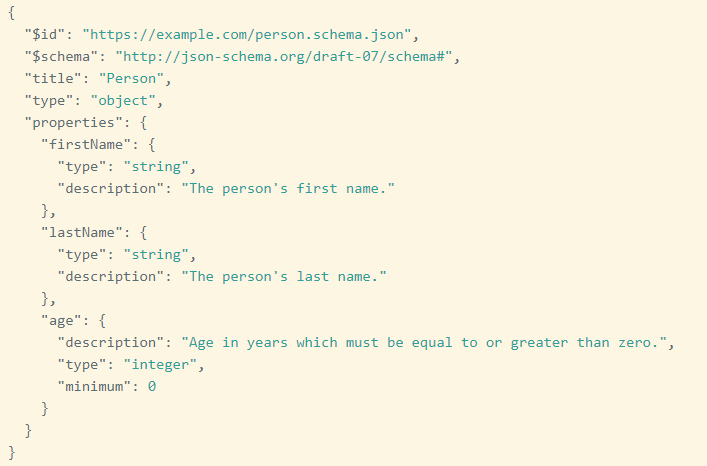
\includegraphics[width=0.4\textwidth]{figures/json_schema_example.png}}
\caption{Example of Json Schema used in OpenAPI \cite{MiscellaneousSchema}}
\label{json_schema_example}
\end{figure}

JSON Schema also allows to "outsoure" the assessment of data categories to professionals. 




For our prototype we are using NodeJS Services

based on Express 

Javascript/Typescript Language for object oriented programmming which provides both typed experience and untyped functions. This will speed up and make. 

As the prototype will not reach production status we do no not need to factor in runtime performances. 

\subsection{Short Introduction to Technologies}




% explain OpenAPI (maybe some history of swagger as well, but not too lengthy) 
% maybe the differences between Swagger(v2) and OpenAPI(v3)? JSONSchema 
% Computer-readable format is needed to be make automated (or semi-automated) processing possible -> OpenAPI is a standard allowing us to describe APIs
% explain tracing frameworks like Zipkin and Jaeger
% explain static analysis
% runtime variables in cloud, eg. location (AWS has variables) 

% Assess practical viability of said technologies

% formulate why we used static analysis or tracing frameworks and which tradeoffs these have
% maybe some usage statistics about OpenAPI / tracking / other tools? How many developers are using it? Is it easy to implement? 
% Why these solutions? What are alternatives and why did we not choose them? 
% Ranking of Tools? 
% How much effort is it? 

% OpenAPI is very versatile: Code can be annotated to generate the specification, but there are also Code generation solutions that generate code from the spec itself.


\subsection{Prototype}
% Provide a (sketchy) outlook about what you are going to implement (esp. your re-usable component)

As described in section \ref{problem} we want to make it easier to track data throughout multiple applications and make it more clear for which purposes . 
We based this on defining the type of data in a central place, which we identiefied as OpenAPI. In order to track data inside of the application we also need a service middleware, which enriches a request with the legal context and logs the type of data transferred. 
Collecting the 
Our Prototype will be set up in a business context. It will simulate a sleep tracking app. Which collects different categories of personal data for different purposes, while being based on a micro-service architecture. 

It will roughly look like the system shown in Figure \ref{prototype_system}

\begin{figure}[htbp]
\centerline{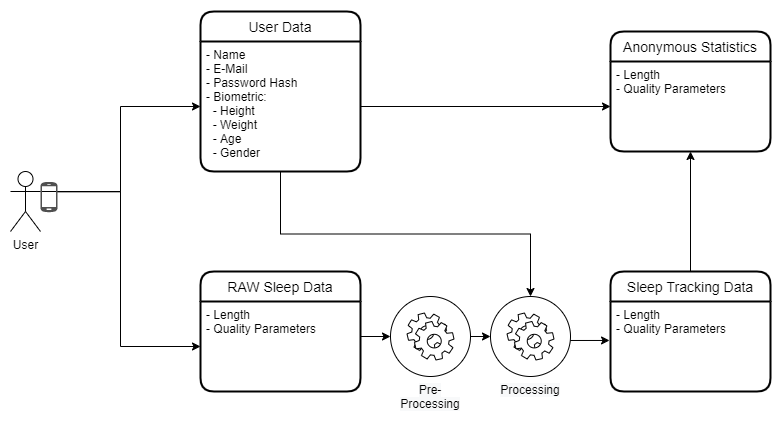
\includegraphics[width=0.4\textwidth]{figures/prototype_system.png}}
\caption{Sketch of our prototype system}
\label{prototype_system}
\end{figure}

Our reusable software components can be split into three main areas: 

\begin{itemize}
    \item Schema Specifications
    \item Service Middleware 
    \item Data collector and analyzer 
\end{itemize}



This could be extended by providing decorators for easier schema specifactions or visualizations for the output data. 
% - Diagramm sketch 
% - flow diagram 

% - Reusable Component: 
%    - OpenAPI Specification based on "Transparency Tracing v2"
%    - Middleware for adding purpose to requests 
%       https://rhonabwy.com/2019/01/06/adding-tracing-with-jaeger-to-an-express-application/
%    - Linter for checking those: https://palantir.github.io/tslint/develop/custom-rules/
%     % https://medium.com/@andrey.igorevich.borisov/writing-custom-tslint-rules-from-scratch-62e7f0237124
%    - Zero Config - Middleware -> % should log to localhost by default? 
    % https://expressjs.com/en/guide/writing-middleware.html
    
    
%    - Visualization of said trace 
%    - Decorator pattern for adding specification easily to OpenAPI % and enable logging itself?
%    - static analysis tool for tracing the data flow

Goals: 

While building a prototype we think that while making something technically feasible it is even more important to make it useful and easily usable. 

Address that services are mostly not microservices in the sense of they fulfill only one purpose (in a GDPR sense) but are fulfilling multiple purposes. e.g. a (example from our system) This has to be taken care of at the application level, for each data request) 

Another pain point is the manual work needed to work with frameworks like yappl which defines a "privacy proxy" which policies assume that the requesting service sends required data like "Institution or Service Name" and "Purpose" in order to enforce the user decision. In future version this could also be extended to related datapoints like "processing-location" "legal-base (and legitimate-interest)" "data-categories" "storage-ttl" "automted-decision-making" \dots .
To this, at the moment the developer has to write and update these strings manually. With out proposed solution this could be partly auto generated.
 
 
 Our approach takes the baseline implementation of \cite{ErnstTransparencyComputing} and updates it to be request specific, while maintaining developer comfort to failback to the centrally provided values. We do this because 
 Because this would lead to the same status quo as before, as nobody would use the optional configuration options we propose a set of easy linting rules which can be applied to each request and inform about more detailed GDPR infos. Another option would be to implement yet another request library to make these required. But in the light of the multitude of availabe languages and the tools available for each language we find that linting rules provide the best approach to be easily rewritten for each tool. 
 The Linter will be based on TSLint which is the standard Linting tool for typescript. 
 
 
 In order to fallback the 
 
 For analyzing purposes we first thought of a static analysis. But this would have several limits. e.g. the used servers (database etc.) are mostly configured at runtime in the production environment. 


Because implementing a Tracing Middleware for each request we might resort to a simpler self-written middleware or mock the responses for the analyzation step. 

During the design of our prototype our subgoal is to not hinder productivity of the developer. 
As this is one of the main pain points in current development \cite{StateDevOps}. 

%Aufgabenstellung: 

Agile DevOps and service-based architectures established as common practice
• Highly dynamic and distributed development, with services being „thrown away“, re-written, and recombined multiple times a day without explicit „waterfall planning“
• Actual and current state of personal data collection, processing and storage hard to be known
• Still, GDPR requires data controllers to be transparent about collection, processing, and use of personal data as well as to maintain respective inventory (records of processing activities),
comprising various information ⟶ Art. 12ff + 30 GDPR
⟶ Employ trace-based approaches, which are widely used in DevOps-settings for gathering overall „state of play“ (and privacy-related interdependencies) in service architectures and for transforming into information required by Art. 12ff + 30 GDPR

Extend an existing tracing system/toolbox of your choice (Jaeger, Zipkin, ...) to allow for trace-based collection of data required by Art. 12ff + 30 GDPR
• Note: This also requires to develop a concept for representing respective information technically (e.g., the purposes for which a certain service processes data) as well as for codifying these into single services – previous work here exists at the ISE chair.
• Provide accompanying tools for executing and utilizing respective tracings for meeting GDPR requirements
• Use your own component for implementing transparency and for auto-generating „records of
processing activities“ a self-chosen, suitable use-case which comprises multiple services, multiple processing purposes and multiple types of personal data
• Extensions: Also consider cross-organizational service invocations etc.

% 3-5 pages not escalated, substantial to the principle we are 
% aware of the correct legal paragraphs 
% supported by law literature

Regarding your further questions:
    2. Is this task more focused on "which data is used where?" (analyze the general personal data flow) or "whose data is used where and when?" (provide a log to the user where his data was processed)

Both options would be valid. Basically, transparency and records of processing only require non-individualized info, but when you propose a technically viable solution for individualization, legal reasoning might come to the conclusion that this (positive) further increase is "reasonable" according to "the state of the art and the cost of implementation" and - tadaaa! - now might become (kind of) obligatory (in certain cases). Independently from that, the general principle of transparency obviously welcomes individualized info independently from what the law (currently) requires in detail. In the end: The more a data subject knows "what data of him/her was used where, how, and by whom for what purpose", the better (and you will have to conduct experiments on the overhead of different levels of detail, selective vs. full take etc. at a later stage). So maybe you just start thinking about how the mentioned question might be answered as far as possible.

    3. Can we ignore (but still state) edge cases or should these be explicitly handled? (e.g. telephone numbers are not always personal data)

Well, I am quite confident that any approach to automatically "detect" personal data will not work because the personal data that is handled in a system can be so manifold. Think a customer id connected to continuously monitored health parameters. These health parameters themselves would clearly be personal data because the controller is able to resolve it to the person. Instead of automatically detecting, I could imagine sth. Like sketched below, but you may very well also come up with completely different approaches - highly welcome.

    4. The task state "This also requires to develop a concept for representing respective information technically (e.g., the purposes for which a certain service processes data) as well as for codifying these into single services"
    What is meant by "codifying these into single services"? Should there be a guarding rail that prohibits services from using some kind of data? Or is this simply referencing service to a certain processing purpose?

What I had in mind here was sth like putting decorators or indicators to the code or some sort of explicit configuration along the implementation. E.g., we had a Master's thesis where the OpenAPI specification of API endpoints could be extended with (schema) elements specifically dedicated to indicating that this endpoint "processes profile data and running routes" serves "the following 3 out of 34 pre-defined purposes". In the attached paper, we rudimentarily sketched sth like this for trace-related configurations (albeit with a way lower complexity than what would be needed in practice). In any case, if you do not come up with a completely different approach (which would, again, be highly welcome), you will presumably need sth like this.





__Tech Report: 

As laid out in the second lesson, the TechReport shall (taking care of the page limit):

Lucas
[I] * (1 Seite) 
Briefly sketch the “privacy principle“ you are about to address with your semester subject (legal grounding is highly welcome)  

% Interesting Link: https://www.i-scoop.eu/gdpr/legal-grounds-lawful-processing-personal-data/
% privacy by transparency art12ff + (evtl. 30??)
% legal ground citations fron gdpr, table from \cite{ErnstTransparencyComputing} extend for location and more detailed description of data we want to collect
% GDPR legal grounding social aspects? 
% name his favourite sentence "if this tech will get mainstream it will be required by law"
% Other legal grounds: California? USA? other 
% Lesson 3: why privacy is a "blurry" concept, "abstract" goals, what societally agreed upon as necessary / helpful principles are 


Lucas 
[II] * (1 Seite) - The Problem 
Describe the particular (still rather generic) technical givens (the use-case) in the light of which you are going to consider and technically address the principle

% Describe current setting (top-down GDPR policies) and current development practices (agile) expressing the need for a better (our) solution
% Different Domains clashing ( Developer <> Data Privacy Law (Jura))
% \cite{ErnstTransparencyComputing} only on service level but reasons should be give more fine grained (e.g. monolithic architecture, not everything is processed with the same purpose
% otherway around data types are the same in a system this don't have to be redefined for each service) 



Piotrek
[III] * (2 Seite) - Particular Challenges of the Problem
Identify (ideally: model) particular challenges arising in this context


% list currently problems, (preferably which will be easier with our setup) 
% many people involved that do not have knowledge of the other domain - our tool should enable (for example) Data Protection Officers to annotate API without them needing to understand the "code" (implementation) 
% mostly manual processes
% gap between user consent and system obligations 
% different law environments (e.g. Europe and California) (ideally the tool should be able to support multiple / we leave this as Future Work)

% Law is specific to a given location and may change over time -> the system should be extensible enough to be able to adapt to the changing environment, but also not to "forget" the past legal environment (even if some things are not required by law anymore)
% - developers have even more things to do, because they now have to specify the GDPR settings as well (with current solutions as well as with our) whats the difference? 

Piotrek / Lucas
[IV] * (2 Seite) - Describe current Solutions to challenges of the problem 
Identify and present the state of scientific discussions with regard to technically addressing the principle in similar/comparable settings

% Explain current solutions in short 
 - privacy languages: 
     - Yappl \cite{Ulbricht2018YaPPLScenarios},
     - TCF: \cite{2019IABFramework-Policies}
 - transparency tracing \cite{ErnstTransparencyComputing},
 - static analysis \cite{Spoto2018StaticCompliance},
 - privacyTracker \cite{2016PrivacyTracker:Controls}
 other papers ?? )


Daniel 
[V] * (1 Seite) - Which tech do we use? What is it? 
Identify and technically describe available technologies that might be used (if any)

% explain OpenAPI (maybe some history of swagger as well, but not too lengthy) 
% maybe the differences between Swagger(v2) and OpenAPI(v3)? JSONSchema 
% Computer-readable format is needed to be make automated (or semi-automated) processing possible -> OpenAPI is a standard allowing us to describe APIs
% explain tracing frameworks like Zipkin and Jaeger
% explain static analysis
% runtime variables in cloud, eg. location (AWS has variables) 

Daniel 
[VI] * (1 Seite) - 
Assess practical viability of said technologies

% formulate why we used static analysis or tracing frameworks and which tradeoffs these have
% maybe some usage statistics about OpenAPI / tracking / other tools? How many developers are using it? Is it easy to implement? 
% Why these solutions? What are alternatives and why did we not choose them? 
% Ranking of Tools? 
% How much effort is it? 

% OpenAPI is very versatile: Code can be annotated to generate the specification, but there are also Code generation solutions that generate code from the spec itself.


Daniel 
[VII] * (2 Seite)
Provide a (sketchy) outlook about what you are going to implement (esp. your re-usable component)

- Diagramm sketch 
- flow diagram 

 - Reusable Component: 
    - OpenAPI Specification based on "Transparency Tracing v2"
      - 
    - Middleware for adding purpose to requests 
    - Linter for checking those: https://palantir.github.io/tslint/develop/custom-rules/
     % https://medium.com/@andrey.igorevich.borisov/writing-custom-tslint-rules-from-scratch-62e7f0237124
    - Zero Config - Middleware -> % should log to localhost by default? 
    % https://expressjs.com/en/guide/writing-middleware.html
    
    
    - Visualization of said trace 
    - Decorator pattern for adding specification easily to OpenAPI % and enable logging itself?
    - static analysis tool for tracing the data flow




Please also have in mind the formal requirements:

*
3-4 (max 5) pages per team member (excluding title, abstract, TOC;
including references)

*
Min 10pt, max 12pt standard font; “reasonable“ margins; justified
typeset; ... (in case of doubt, use established template, e.g., Springer,
IEEE, ...)


Notizen: 
Hauptaugenmerk auf technischer Implementierung --> cooles Stück Code umso näher an tatsächlicher Umgenbung umso besser

- mehrere Sevices die ineinander greifen und sich gegenseitig aufrufen um die Verschachtelung aufzuzeigen
User-Zentraldatenbanken (Stammdaten, Conten-Data) 


- Abgabe auf English 
- Zu Sketchy, was macht ihr eigentlich? 
- komplexere Services 
- Demo für letzendliche Präsentation
- Generierung von Übersicht

Wunsch: 
 - mehr Content! 
   - das lässt sich einsetzen
 - 
  

\printglossaries
\bibliographystyle{IEEEtran}
\bibliography{references}

\end{document}
